% =====================================================================
%  A Physics-Guided Digital Twin Framework for Urban Infrastructure
%  Resilience Assessment under Extreme Flooding
%
%  Compiled with: pdflatex manuscript (bibtex, pdflatex x2)
%  Journal format: Elsevier elsarticle (generic; adjust options for the
%  target journal, e.g. \documentclass[preprint,12pt]{elsarticle})
% =====================================================================
\documentclass[preprint,12pt]{elsarticle}

\usepackage{amsmath,amssymb}
\usepackage{booktabs}
\usepackage{graphicx}
\usepackage{multirow}
\usepackage{algorithm}
\usepackage{algpseudocode}
\usepackage[colorlinks=true,linkcolor=blue,citecolor=blue,urlcolor=blue]{hyperref}

\journal{}

\begin{document}

\begin{frontmatter}

\title{A Physics-Guided Digital Twin Framework for Urban Infrastructure
Resilience Assessment under Extreme Flooding: Integrating Terrain-Informed
Flood Simulation, Delayed Cascading Failures, and Adaptive Restoration}

\author[aff1]{Zheyu Huang\corref{cor1}}
\ead{zheyu.huang@example.edu}
\author[aff2]{Yujia Huang}
\cortext[cor1]{Corresponding author.}
\affiliation[aff1]{organization={Department of Civil and Environmental
Engineering, University of Example}, city={Example City}, country={Country}}
\affiliation[aff2]{organization={School of Urban Planning, Example Institute},
city={Example City}, country={Country}}

\begin{abstract}
Extreme flooding poses increasing risks to urban systems due to the combined
impacts of climate change, rapid urbanization, and growing interdependencies
among critical infrastructures. Existing urban resilience assessment
approaches predominantly rely on static vulnerability indicators or isolated
infrastructure analysis, which are insufficient to capture the dynamic
evolution of flood hazards, cascading failures, and adaptive recovery
processes. To address this limitation, this study proposes a physics-guided
digital twin framework for dynamic urban flood resilience assessment and
adaptive recovery optimization.

The proposed framework integrates four coupled components: (1) a
terrain-informed cellular flood simulation model for high-resolution hazard
evolution, (2) a multi-layer infrastructure network model for representing
interdependent system behavior, (3) a time-delayed cascading failure analysis
for capturing failure propagation among power and communication
infrastructures, and (4) an adaptive restoration optimization module for
supporting dynamic emergency response decisions under flood-constrained
transportation. A spatiotemporal digital twin environment is developed to
continuously update urban system states by coupling physical hazard
processes, infrastructure conditions, and recovery strategies.

A case study of Miyazaki City, Japan, is conducted to evaluate the proposed
framework under an extreme typhoon rainfall scenario with a peak intensity of
100~mm/h. The results demonstrate that the framework can effectively
reproduce nonlinear flood propagation driven by heterogeneous terrain and
drainage saturation, identify spatial distributions of infrastructure
exposure, and reveal delayed cascading failure mechanisms caused by
infrastructure interdependencies and backup-energy depletion. Compared with
conventional fixed-priority restoration strategies and non-intervention
scenarios, the proposed adaptive restoration approach improves recovery
efficiency by dynamically allocating limited repair resources according to
system conditions and infrastructure criticality. Sensitivity analyses
further highlight the significant effects of rainfall intensity, drainage
capacity, backup-battery duration, and repair-resource availability on urban
resilience performance.

This study contributes a comprehensive and computationally reproducible
digital twin framework that bridges physical flood modeling, infrastructure
resilience analysis, and intelligent recovery decision-making. The proposed
approach provides a practical foundation for next-generation urban resilience
planning, emergency management, and climate adaptation under increasing flood
risks.
\end{abstract}

\begin{keyword}
Urban resilience \sep Digital twin \sep Cellular automata flood simulation
\sep Interdependent infrastructure networks \sep Cascading failures
\sep Adaptive restoration \sep Critical infrastructure protection
\end{keyword}

\end{frontmatter}

% =====================================================================
\section{Introduction}\label{sec:intro}

Climate change has intensified the frequency and severity of extreme
precipitation events, making urban flooding one of the most significant
threats to sustainable urban development~\cite{ipcc2012srex}. Unlike
conventional natural hazards that affect isolated components, extreme floods
increasingly interact with interconnected urban infrastructure systems,
including power supply networks, communication networks, transportation
systems, and water management facilities~\cite{rinaldi2001identifying}. The
increasing dependence among these systems introduces complex failure
propagation mechanisms, where localized physical damage can trigger
large-scale cascading disruptions across multiple infrastructure
domains~\cite{buldyrev2010catastrophic,gao2011robustness}.

Critical infrastructure systems (CIS) are characterized by strong physical
and functional interdependencies. For example, communication networks rely
on continuous power supply, while emergency response activities require
functioning transportation systems~\cite{ouyang2014review}. Consequently,
failures occurring in one infrastructure layer may propagate into other
layers through dependency relationships, potentially leading to nonlinear
system degradation and prolonged recovery periods~\cite{ouyang2012three}.
Therefore, accurately evaluating infrastructure resilience requires not only
identifying vulnerable components but also reproducing the dynamic
interactions among hazards, infrastructure failures, and recovery
interventions~\cite{bruneau2003framework,chang2004measuring}.

Existing studies have investigated infrastructure vulnerability and cascading
failures from various perspectives. Complex network theory and
percolation-based approaches have provided valuable insights into the
structural robustness of interdependent
networks~\cite{albert2002statistical,newman2003structure,gao2011robustness}.
However, many existing models simplify disaster impacts as instantaneous node
failures or probabilistic disturbances, without explicitly considering the
underlying physical processes that generate infrastructure damage. Such
simplifications may result in inaccurate estimation of failure timing and
system-level resilience~\cite{ouyang2012time}.

One major limitation concerns the representation of flood hazards. Many urban
flood resilience studies adopt simplified approaches such as bathtub models,
uniform water-level assumptions, or distance-based hazard indicators.
Although computationally efficient, these approaches neglect the influence of
heterogeneous urban topography, surface runoff pathways, and nonlinear
drainage limitations~\cite{bates2010simple}. In reality, flood propagation is
governed by complex interactions among rainfall intensity, terrain gradients,
drainage capacity, and local accumulation processes~\cite{guidolin2016weighted,
ghimire2013formulation}. Without a physically informed hydrodynamic
representation, it remains difficult to identify critical transition points
where urban flooding rapidly evolves from a manageable condition into a
catastrophic state.

Another limitation lies in the temporal characteristics of infrastructure
failure. Conventional cascading failure models frequently assume immediate
failure propagation after dependency loss~\cite{buldyrev2010catastrophic}.
However, practical infrastructure systems often contain redundancy mechanisms
that provide temporary operational capability. For instance, communication
facilities are commonly equipped with backup batteries or uninterrupted power
supply systems. When external power sources fail, these facilities may
continue operating for a limited period before complete shutdown
~\cite{panteli2015grid}. This delayed failure mechanism introduces an
important resilience buffer, creating a temporal window for emergency
intervention. Nevertheless, the impact of such time-dependent degradation
processes remains insufficiently explored in existing interdependent
infrastructure models.

Furthermore, many current digital twin and resilience assessment frameworks
primarily focus on damage simulation while neglecting the active role of
emergency restoration~\cite{batty2018digital,grieves2017digital,
tao2019digital}. In real disaster scenarios, recovery operations occur within
rapidly changing physical environments. Floodwaters may dynamically block
transportation networks, alter travel accessibility, and increase response
delays~\cite{laporte2009fifty}. Therefore, emergency dispatch decisions
should not rely solely on static road networks or geographical distances.
Instead, restoration strategies should incorporate real-time environmental
conditions and adaptive routing mechanisms to capture the interaction between
disaster evolution and human intervention~\cite{dibaldassarre2013socio}.

To address these limitations, this study develops a high-resolution
four-dimensional digital twin framework that integrates physical flood
dynamics, infrastructure interdependency, and adaptive restoration processes
within a unified simulation environment. The framework combines a
terrain-informed cellular automata (CA) flood propagation model with
interdependent network failure modeling and dynamic emergency dispatch
optimization. Compared with previous studies focusing separately on flood
simulation, infrastructure vulnerability, or restoration planning, the
proposed approach enables closed-loop analysis of hazard evolution, cascading
failures, and recovery actions.

The main contributions of this study are summarized as follows:
\begin{itemize}
\item \textbf{High-resolution flood dynamics modeling.} A terrain-informed
cellular automata flood propagation model is developed using high-resolution
elevation data. The model incorporates heterogeneous drainage capacity and
subsurface storage limitations to reproduce nonlinear urban flood evolution
and identify critical flooding transition points.
\item \textbf{Time-delayed cascading failure mechanism.} A coupled
power--communication infrastructure model is proposed by integrating
flood-induced physical damage with backup-battery depletion dynamics. This
approach captures delayed failure propagation and reveals the temporal
characteristics of cascading disruptions.
\item \textbf{Dynamic restoration optimization under flood constraints.} A
human-in-the-loop restoration mechanism is introduced by coupling
flood-dependent road accessibility, dynamic shortest-path routing, and
multi-objective emergency prioritization. The proposed strategy evaluates how
adaptive interventions influence infrastructure resilience during disaster
evolution.
\end{itemize}

The remainder of this paper is organized as follows. Section~\ref{sec:rw}
reviews related studies on digital twins, flood simulation, infrastructure
interdependency, and resilience assessment. Section~\ref{sec:method}
presents the proposed digital twin framework and mathematical formulations.
Section~\ref{sec:case} introduces the case study and experimental design.
Section~\ref{sec:results} discusses simulation results and comparative
analyses. Section~\ref{sec:discussion} provides further discussion of
practical implications and limitations. Finally, Section~\ref{sec:conclusion}
concludes the study and highlights future research directions.

% =====================================================================
\section{Related Work}\label{sec:rw}

\subsection{Digital Twins in Urban Disaster Management}
Digital twin technology has emerged as an effective approach for representing
complex urban systems by integrating physical entities, sensing data,
computational models, and decision-support mechanisms~\cite{grieves2017digital,
tao2019digital}. In recent years, urban digital twins have been increasingly
applied in infrastructure monitoring, smart city management, and disaster
response due to their capability to provide continuous system-state
representation and scenario-based analysis~\cite{batty2018digital}.

Existing studies have demonstrated the potential of digital twins in
improving situational awareness during urban emergencies. By integrating
geographic information systems (GIS), Internet of Things (IoT) observations,
and simulation models, digital twin platforms can support real-time
visualization and decision-making for complex urban environments
~\cite{haklay2008openstreetmap}. However, many current urban digital twin
applications primarily focus on data integration, visualization, and asset
management, while the dynamic coupling between hazard evolution and
infrastructure response remains insufficiently explored. For flood resilience
assessment, an effective digital twin should not only reproduce the spatial
distribution of hazards but also capture the temporal interactions between
environmental processes, infrastructure degradation, and recovery actions.

\subsection{Flood Simulation and Urban Flood Dynamics Modeling}
Urban flood simulation has been widely investigated using hydrodynamic
models, cellular automata approaches, and hybrid modeling techniques.
Traditional hydrodynamic models based on shallow-water equations (SWE) can
provide physically meaningful flood propagation simulations
~\cite{bates2010simple}; however, they often require detailed hydraulic
parameters and considerable computational resources, limiting their
application in large-scale real-time digital twin environments.

Cellular automata-based flood models have attracted increasing attention due
to their computational efficiency and capability of representing spatially
distributed flood evolution~\cite{ghimire2013formulation,
guidolin2016weighted,issermann2020efficient}. By defining local transition
rules among neighboring cells, CA models can effectively simulate inundation
propagation, water accumulation, and terrain-driven flow behaviors. However,
existing CA-based approaches are often developed independently from
infrastructure systems and mainly focus on flood extent prediction rather
than disaster-induced functional degradation. Consequently, there remains a
need for integrated approaches that couple flood propagation processes with
infrastructure functional states within a unified simulation framework.

\subsection{Cascading Failure Modeling in Interdependent Infrastructure Networks}
Modern cities rely on highly interconnected infrastructure networks,
including power systems, communication networks, transportation systems, and
water supply systems~\cite{rinaldi2001identifying}. Such interdependencies
improve operational efficiency but also increase vulnerability to cascading
failures during extreme events~\cite{buldyrev2010catastrophic,gao2011robustness}.

Previous studies have developed various network-based approaches to analyze
cascading failures, including graph theory models, percolation theory,
agent-based simulations, and reliability-based approaches
~\cite{ouyang2014review}. These methods have significantly improved the
understanding of infrastructure vulnerability under disruptive events.
However, several limitations remain. First, many existing studies assume that
failures occur instantaneously after component damage, neglecting temporal
delays associated with degradation, backup operation, and maintenance
response~\cite{ouyang2012time}. Second, infrastructure networks are
frequently analyzed independently, while real urban systems exhibit complex
cross-network dependencies~\cite{ouyang2012three}. Third, most existing
models focus on failure propagation but provide limited integration with
recovery decision-making processes.

\subsection{Resilience Assessment and Adaptive Recovery Optimization}
Urban resilience has evolved from a concept focusing on resistance and
robustness toward a broader perspective incorporating absorption, adaptation,
and recovery capabilities~\cite{holling1973resilience,bruneau2003framework}.
Existing resilience assessment methods commonly use performance-based
indicators, resilience curves, vulnerability indices, and recovery
trajectories to quantify system performance during disruptive
events~\cite{chang2004measuring,ouyang2012three}.

Although these approaches provide valuable evaluation frameworks, recovery
planning is often treated as an independent optimization problem after
disaster occurrence~\cite{ouyang2012time}. In reality, restoration decisions
should continuously adapt to evolving system conditions, resource
limitations, accessibility constraints, and infrastructure criticality
~\cite{laporte2009fifty}. Recent studies have explored optimization-based
recovery strategies using heuristic algorithms and network centrality
analysis. Nevertheless, many approaches rely on predefined priorities and
lack real-time interaction with hazard evolution models. Integrating adaptive
restoration optimization into a dynamic digital twin environment remains an
open research direction.

\subsection{Research Gaps and Motivation}
Based on the above review, three major research gaps are identified. First,
existing urban digital twin studies mainly emphasize data integration and
visualization, while insufficient attention has been given to coupling
physical hazard evolution with infrastructure functional dynamics. Second,
current flood simulation and infrastructure resilience models are often
developed separately, limiting their capability to represent flood-induced
cascading failures across interdependent urban systems. Third, existing
recovery optimization methods generally rely on static strategies and do not
dynamically adapt to changing disaster conditions. To address these
limitations, this study develops a physics-guided spatiotemporal digital twin
framework that integrates flood propagation modeling, interdependent
infrastructure failure simulation, and adaptive restoration optimization.

% =====================================================================
\section{Methodology}\label{sec:method}

\subsection{Overview of the Proposed Digital Twin Framework}
This study develops a physics-informed high-resolution digital twin framework
for assessing urban infrastructure resilience under extreme flooding events.
The proposed framework integrates three coupled components: (1) a
terrain-driven flood evolution model based on cellular automata, (2) an
interdependent infrastructure failure model incorporating time-delayed
cascading effects, and (3) a dynamic restoration optimization module
considering flood-induced transportation constraints.

The overall simulation framework follows a closed-loop disaster-response
process. At each simulation cycle, rainfall forcing is first introduced into
the physical environment. The CA-based flood model then updates the spatial
flood distribution by considering terrain characteristics, water exchange
among neighboring cells, and heterogeneous drainage responses. The resulting
flood field determines the physical status of infrastructure components,
including power substations and communication facilities. Subsequently,
cascading failure dynamics are calculated through dependency relationships
between infrastructure layers. Finally, emergency restoration decisions are
generated according to current network conditions and dynamic transportation
accessibility. The complete interaction process is expressed as:
\begin{equation}\label{eq:loop}
\text{Rainfall} \rightarrow \text{Flood evolution} \rightarrow
\text{Infrastructure damage} \rightarrow \text{Cascading failure}
\rightarrow \text{Dynamic restoration} \rightarrow
\text{Resilience update}.
\end{equation}

This multi-layer coupling enables the proposed digital twin to reproduce not
only disaster-induced physical degradation but also the adaptive responses of
urban systems during recovery.

\subsection{Terrain Reconstruction and Physical Environment Model}
To capture the influence of urban micro-topography on flood propagation, the
study area is discretized into a two-dimensional regular cellular grid:
\begin{equation}\label{eq:grid}
\mathbf{C} = \{C(i,j) \mid i=1,\dots,N_x,\ j=1,\dots,N_y\},
\end{equation}
where each cell $C(i,j)$ represents a spatial unit with horizontal
resolutions $\Delta x$ and $\Delta y$. In the case study the computational
domain consists of $N_x=N_y=650$ cells, resulting in 422{,}500 spatial
cells.

The original terrain elevation data are reconstructed into a continuous
elevation matrix $\mathbf{Z}_0 \in \mathbb{R}^{N_x\times N_y}$ through spatial
interpolation. To reduce interpolation noise while preserving important
terrain gradients, a Gaussian smoothing operator is applied:
\begin{equation}\label{eq:smooth}
Z(i,j) = (G_\sigma * Z_0)(i,j),
\end{equation}
where $G_\sigma$ denotes the Gaussian kernel and $\sigma$ controls the
smoothing intensity ($\sigma=0.8$ in this study).

Local terrain gradients determine the preferential direction of surface water
movement. The spatial gradient is estimated using second-order central
differences, and the local slope magnitude is calculated as:
\begin{equation}\label{eq:slope}
S(i,j) = \sqrt{\left(\frac{\partial Z}{\partial x}\right)^2 +
\left(\frac{\partial Z}{\partial y}\right)^2},
\end{equation}
which is normalized to $\hat{S}(i,j)\in[0,1]$ by min--max scaling. The
normalized slope field drives the spatial heterogeneity of drainage
capacity and subsurface storage described below.

\subsection{Terrain-Informed Cellular Flood Propagation Model}
\subsubsection{Model principles}
Full numerical solutions of the shallow water equations provide high physical
accuracy but become computationally expensive for large-scale urban
simulations with fine spatial resolution~\cite{bates2010simple}. This study
therefore adopts a cellular automata-based flood propagation approximation
that follows three principles: (i) local mass conservation between
neighboring cells; (ii) gravity-driven water redistribution according to
hydraulic head differences; and (iii) adaptive drainage response constrained
by local environmental characteristics~\cite{ghimire2013formulation,
guidolin2016weighted}.

\subsubsection{Rainfall input and hydraulic head}
The rainfall intensity is converted into water depth increments:
\begin{equation}\label{eq:rain}
W^{*}(i,j,t) = W(i,j,t) + R(t),
\end{equation}
where $W(i,j,t)$ is the surface water depth and $R(t)$ the rainfall depth
increment per time step. The hydraulic head of each cell is:
\begin{equation}\label{eq:head}
H(i,j,t) = Z(i,j) + W^{*}(i,j,t).
\end{equation}

\subsubsection{Hydraulic flux exchange between cells}
For each neighboring direction $d \in \Omega = \{\mathrm{N,S,E,W}\}$, the
positive hydraulic head difference is
$\Delta H_d^{+}(i,j,t) = \max(0,\, H(i,j,t) - H_d(i,j,t))$, and the total
available gradient is $\Delta H_{\mathrm{total}} =
\sum_{d\in\Omega}\Delta H_d^{+}$. The maximum transferable water volume is
constrained by the flux limitation coefficient $\alpha$:
\begin{equation}\label{eq:qlim}
Q_{\mathrm{lim}}(i,j,t) = \alpha\, W^{*}(i,j,t),
\end{equation}
and the directional flux is allocated proportionally to the head differences:
\begin{equation}\label{eq:qdir}
Q_d(i,j,t) =
\begin{cases}
\dfrac{\Delta H_d^{+}}{\Delta H_{\mathrm{total}}}\, Q_{\mathrm{lim}},
& \Delta H_{\mathrm{total}} > 0,\\[4pt]
0, & \Delta H_{\mathrm{total}} = 0.
\end{cases}
\end{equation}
According to the Courant--Friedrichs--Lewy (CFL) stability condition, the
outflow coefficient must satisfy $4\alpha \le 1$; we conservatively set
$\alpha = 0.12$.

\subsubsection{Drainage response and storage saturation}
Urban drainage capability is spatially heterogeneous. The effective drainage
rate is defined as:
\begin{equation}\label{eq:drain}
D(i,j) = D_0\,\bigl(1 + \eta\,\hat{S}(i,j)\bigr),
\end{equation}
where $D_0$ is the basic drainage capacity and $\eta$ the terrain-dependent
response intensity. The available subsurface storage capacity $K(i,j,t)$
decreases as water is drained, and the actual drainage volume is constrained
by water availability, drainage rate, and remaining storage:
\begin{equation}\label{eq:dact}
D_{\mathrm{act}}(i,j,t) =
\min\!\bigl(W^{*}(i,j,t),\ D(i,j)\,\Delta t,\ K(i,j,t)\bigr),
\end{equation}
with the storage evolution
\begin{equation}\label{eq:storage}
K(i,j,t+\Delta t) = \max\!\bigl(0,\ K(i,j,t) - D_{\mathrm{act}}(i,j,t)\bigr).
\end{equation}
When $K(i,j,t)=0$, the drainage system reaches saturation and additional
rainfall contributes directly to surface flooding, generating a nonlinear
tipping point in flood evolution.

\subsubsection{Water depth evolution}
Considering incoming flux, outgoing flux, and drainage removal, the water
depth update equation is:
\begin{equation}\label{eq:update}
W(i,j,t+\Delta t) = W(i,j,t) - \sum_{d} Q_d^{\mathrm{out}} +
\sum_{d} Q_d^{\mathrm{in}} - D_{\mathrm{act}}(i,j,t),
\end{equation}
which ensures local mass conservation while allowing efficient large-scale
flood evolution simulation.

\subsection{Time-Delayed Cascading Failure Model in Interdependent Networks}
\subsubsection{Interdependent network representation}
Urban critical infrastructure systems are modeled as interdependent
multi-layer networks consisting of a power supply layer $G_p = (P, E_p)$,
where $P = \{p_1,\dots,p_M\}$ denotes power substations, and a communication
layer $G_c = (C, E_c)$, where $C = \{c_1,\dots,c_N\}$ denotes communication
base stations. A dependency mapping $f_{\mathrm{dep}}: C \rightarrow P$
assigns each communication node to one upstream power node. Unlike purely
geographical dependency assumptions, dependencies are established according
to network accessibility:
\begin{equation}\label{eq:dep}
f_{\mathrm{dep}}(c_i) = \arg\min_{p_j \in P}\,
\mathrm{Dist}_{\mathcal{G}}(c_i, p_j),
\end{equation}
where $\mathrm{Dist}_{\mathcal{G}}$ is the shortest infrastructure
connection distance.

\subsubsection{Flood-induced physical failure of power infrastructure}
For each power substation $p_j$, the local flood depth
$W_p(p_j,t) = W(x_{p_j}, y_{p_j}, t)$ is sampled from the hydrodynamic field.
The operational state $S_p(p_j,t)\in\{0,1\}$ follows a threshold mechanism:
\begin{equation}\label{eq:pfail}
S_p(p_j,t) =
\begin{cases}
1, & W_p(p_j,t) \le W_{\mathrm{th}},\\
0, & W_p(p_j,t) > W_{\mathrm{th}},
\end{cases}
\end{equation}
where $W_{\mathrm{th}} = 0.5$~m is the flood tolerance threshold of
substations. Physical flood damage is assumed irreversible without external
restoration intervention: $S_p(p_j,t+\Delta t) \le S_p(p_j,t)$ unless a
repair action is completed.

\subsubsection{Time-delayed failure propagation through backup energy}
A key feature of urban infrastructure resilience is that dependency failure
does not always propagate instantaneously. Communication nodes are equipped
with backup batteries whose initial capacity follows
$B(c_i,0) \sim U(B_{\min}, B_{\max})$ (here 3--5~h). When the associated power
node fails, battery depletion begins:
\begin{equation}\label{eq:battery}
B(c_i,t+\Delta t) =
\max\!\left[0,\ B(c_i,t) -
\lambda\,\bigl(1 - S_p(f_{\mathrm{dep}}(c_i),t)\bigr)\,\Delta t\right],
\end{equation}
where $\lambda$ is the normalized battery consumption rate. The communication
node operational state is $S_c(c_i,t) = 1$ if $B(c_i,t) > 0$ and $0$
otherwise. This formulation introduces a temporal buffer between physical
damage and functional failure, enabling the model to capture delayed cascading
effects.

\subsection{Dynamic Restoration Optimization under Flood-Constrained Transportation}
\subsubsection{Flood-dependent dynamic road network}
The urban road system is modeled as a dynamic weighted graph
$G_r(t) = (V, E, L(t))$, where $L(t)$ is the time-dependent travel cost. For a
road segment $e_{uv}$, the flood condition is sampled at its geometric
center, $W_r(e_{uv},t)$, and the dynamic travel impedance is:
\begin{equation}\label{eq:road}
L(u,v,t) =
\begin{cases}
L_0(u,v), & W_r(e_{uv},t) \le W_{\mathrm{road}},\\
\infty, & W_r(e_{uv},t) > W_{\mathrm{road}},
\end{cases}
\end{equation}
where $W_{\mathrm{road}} = 0.3$~m is the maximum safe water depth for
emergency vehicles.

\subsubsection{Multi-objective restoration priority}
Restoring a substation with many dependent communication nodes can recover
more network functionality, while nodes approaching battery depletion require
urgent intervention. A restoration utility function is therefore defined:
\begin{equation}\label{eq:utility}
U(p_j,t) = \sum_{c_i \in C(p_j)}
S_c(c_i,t)\left(1 + \frac{\gamma}{B(c_i,t)+\epsilon}\right),
\end{equation}
where $C(p_j)$ denotes the communication nodes dependent on substation $p_j$,
$\gamma$ controls urgency sensitivity, and $\epsilon$ avoids numerical
singularity. The optimal restoration target is selected as
$p^{*} = \arg\max_{p_j} U(p_j,t)$.

\subsubsection{Dynamic shortest-path routing and restoration}
After selecting a restoration target, repair fleet $f_k$ searches for the
optimal route under the current road condition:
\begin{equation}\label{eq:routing}
\Pi_k^{*}(t) = \arg\min_{\Pi} \sum_{(u,v)\in\Pi} L(u,v,t),
\end{equation}
solved with the Dijkstra algorithm. When the fleet reaches the failed power
node at time $t_{\mathrm{arrive}}$, the restoration action is activated,
$S_p(p^{*}, t_{\mathrm{arrive}}) \rightarrow 1$, which immediately stops the
battery depletion of its dependent communication nodes and prevents further
cascading failure.

\subsection{Simulation Workflow}
The complete simulation process is summarized in
Algorithm~\ref{alg:digital_twin}. The system resilience indicator
$\Phi(t) = \frac{1}{N}\sum_{i=1}^{N} S_c(c_i,t)$ tracks the fraction of
operational communication nodes over time.

\begin{algorithm}[H]
\caption{High-resolution urban resilience digital twin simulation}
\label{alg:digital_twin}
\begin{algorithmic}[1]
\State Initialize terrain elevation, drainage parameters, and infrastructure networks
\For{each simulation timestep $t$}
  \State Update rainfall forcing
  \State Calculate CA-based flood propagation (Eq.~\ref{eq:update})
  \State Update drainage storage saturation (Eq.~\ref{eq:storage})
  \State Evaluate power infrastructure flooding damage (Eq.~\ref{eq:pfail})
  \State Update communication battery depletion (Eq.~\ref{eq:battery})
  \State Calculate system resilience indicator $\Phi(t)$
  \If{failed infrastructure exists}
    \State Compute restoration priorities (Eq.~\ref{eq:utility})
    \State Update dynamic road accessibility (Eq.~\ref{eq:road})
    \State Generate optimal repair routes (Eq.~\ref{eq:routing})
    \State Execute restoration actions
  \EndIf
\EndFor
\State Output flood evolution and resilience trajectories
\end{algorithmic}
\end{algorithm}

% =====================================================================
\section{Case Study and Experimental Design}\label{sec:case}

\subsection{Study Area}
To evaluate the effectiveness of the proposed digital twin framework, a case
study was conducted in Miyazaki City, Japan. Miyazaki City is located on the
southeastern coast of Kyushu Island and is frequently affected by
typhoon-induced extreme precipitation events. The urban area is characterized
by heterogeneous terrain conditions, including elevated mountainous regions
in the west and relatively flat low-elevation plains near the Pacific
coastline. The Oyodo River system crosses the urban area, creating complex
surface runoff patterns and flood accumulation zones. The combination of
mountainous runoff generation and low-elevation urban development makes
Miyazaki City an appropriate testbed for evaluating terrain-driven flood
dynamics and infrastructure resilience under extreme rainfall conditions.

\subsection{Digital Twin Environment Construction}
\subsubsection{Terrain and hydrological data}
The physical environment was reconstructed using high-resolution elevation
data obtained from open geographic databases (Open-Meteo elevation API). The
road network within a 3~km radius of the city center was extracted from
OpenStreetMap~\cite{haklay2008openstreetmap} and projected to the local
coordinate system EPSG:6674 for accurate distance computation. The study
region was discretized into a $650\times650$ cell computational domain
(422{,}500 hydrological cells), each containing elevation, surface water
depth, drainage capacity, and subsurface storage state. The terrain field was
processed using Gaussian smoothing to remove interpolation artifacts while
preserving local elevation variations.

\subsubsection{Infrastructure network initialization}
Two critical infrastructure layers were constructed: a power supply network
with $M=15$ substations and a communication network with $N=40$ base
stations. Dependency relationships were established according to
network-based shortest-path distance rather than Euclidean distance,
reflecting the practical characteristics of urban infrastructure
connectivity~\cite{rinaldi2001identifying}. Table~\ref{tab:data} summarizes
the input datasets.

\begin{table}[H]
\centering
\caption{Data sources used in the digital twin framework}
\label{tab:data}
\begin{tabular}{lll}
\toprule
Dataset & Purpose & Model component \\
\midrule
Open-Meteo elevation API & Terrain reconstruction and slope & Flood model \\
OpenStreetMap road network & Topology and accessibility & Network model \\
Infrastructure deployment & Component failure analysis & Cascading failure model \\
Synthetic rainfall scenario & Hazard forcing & Flood model \\
Recovery parameters & Emergency response & Restoration optimization \\
\bottomrule
\end{tabular}
\end{table}

\subsection{Extreme Rainfall Scenario}
An extreme rainfall event lasting $T=8$~h was simulated. The rainfall input
followed a modified Chicago design storm profile:
\begin{equation}\label{eq:rainfall}
R(t) = R_{\mathrm{base}} + R_{\mathrm{peak}} \sin\!\left(\frac{\pi t}{T}\right),
\end{equation}
with a peak intensity of 100~mm/h and a cumulative precipitation of
approximately 567~mm. The scenario represents a severe typhoon precipitation
event comparable with historical extreme rainfall conditions in southern
Japan. The time axis was discretized into 24 frames, each containing 30 CA
sub-steps of $\Delta t = 10$~s.

\subsection{Simulation Parameters}
The main simulation parameters are summarized in
Table~\ref{tab:parameters}.

\begin{table}[H]
\centering
\caption{Main simulation parameters}
\label{tab:parameters}
\begin{tabular}{lll}
\toprule
Category & Parameter & Value \\
\midrule
Spatial resolution & Grid size & $650\times650$ \\
Flood model & Cell number & 422{,}500 \\
Rainfall & Duration & 8~h \\
Rainfall & Peak intensity & 100~mm/h \\
Infrastructure & Power substations & 15 \\
Infrastructure & Communication stations & 40 \\
Flood threshold & Substation damage threshold & 0.5~m \\
Transportation & Road blockage threshold & 0.3~m \\
Battery & Backup duration & 3--5~h \\
Restoration & Repair fleets & 2 \\
Restoration & Fleet speed & 30~km/h \\
Restoration & Repair time per substation & 1~h \\
\bottomrule
\end{tabular}
\end{table}

\subsection{Experimental Scenarios and Evaluation Metrics}
Four experimental scenarios were designed to evaluate different capabilities
of the proposed framework: \textbf{S1} normal rainfall condition (baseline
for normal system behavior); \textbf{S2} extreme flood scenario (main
scenario, evaluating flood propagation and infrastructure exposure);
\textbf{S3} infrastructure cascading failure scenario (activating
interdependency mechanisms); and \textbf{S4} adaptive restoration comparison
(comparing adaptive restoration with static-flood and no-restoration
baselines).

Two baselines were defined for ablation analysis:
\begin{itemize}
\item \textbf{Baseline 1 (static bathtub flood).} The CA flood model is
replaced by a spatially uniform accumulation model in which the drainage
coefficient is fixed at the median of the heterogeneous drainage field,
$D_{\mathrm{const}} = \mathrm{median}(D(i,j))$. This represents simplified
flood assessment approaches that neglect heterogeneous terrain effects.
\item \textbf{Baseline 2 (no restoration intervention).} The proposed flood
and cascading failure mechanisms are preserved, but emergency dispatch
actions are removed ($K=0$ fleets); failed infrastructure remains
unrecovered throughout the simulation.
\end{itemize}

The performance of the framework is evaluated with four indicators:
(i) flood extent and depth distribution, (ii) the resilience index
$\Phi(t)$ and its time integral (resilience area under the curve, AUC),
(iii) recovery time (first time at which $\Phi(t)$ returns to 95\% of its
initial value), and (iv) infrastructure availability curves
$A(t) = N_{\mathrm{functional}}(t)/N_{\mathrm{total}}$.

% =====================================================================
\section{Results and Performance Evaluation}\label{sec:results}

\subsection{Study Area and Infrastructure Deployment}
Fig.~\ref{fig:studyarea} shows the reconstructed terrain of the study area
together with the OSM road network and the deployed infrastructure. The
western mountainous region and the eastern coastal plain are clearly
distinguished, providing a heterogeneous physical basis for flood
propagation.

\begin{figure}[H]
\centering
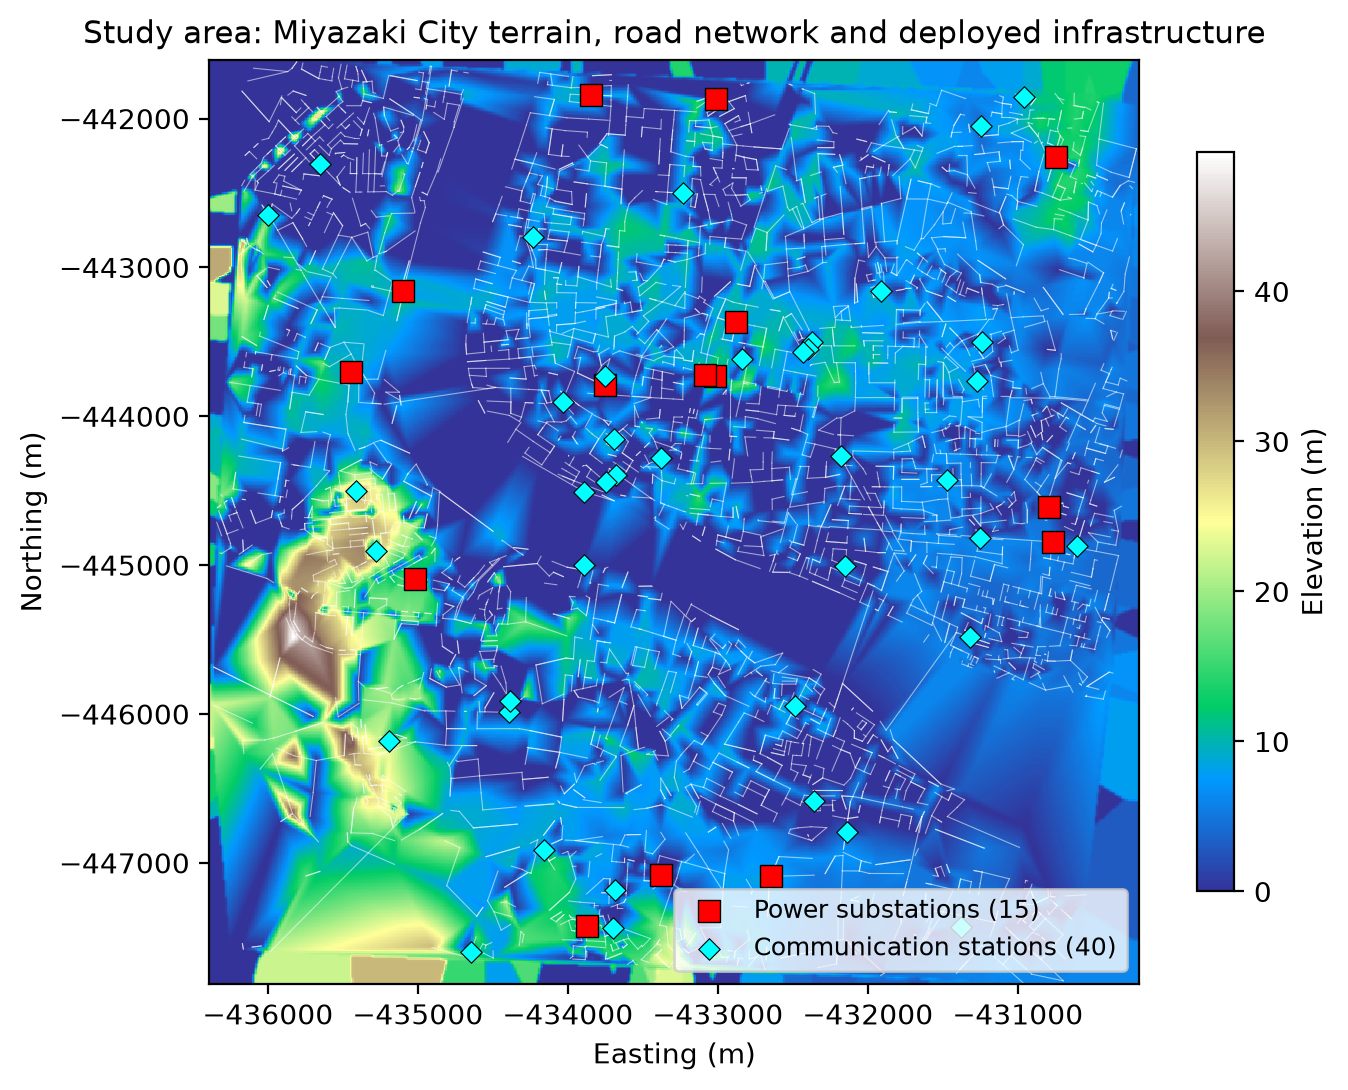
\includegraphics[width=0.92\linewidth]{figures/fig1_study_area.png}
\caption{Study area (Miyazaki City): reconstructed terrain, road network, and
deployed power substations (red squares) and communication base stations
(cyan diamonds).}
\label{fig:studyarea}
\end{figure}

\subsection{Nonlinear Flood Evolution and Drainage Saturation}
The proposed CA flood simulation reveals a nonlinear flood evolution process
caused by interactions among rainfall intensity, terrain characteristics, and
drainage limitations. Fig.~\ref{fig:flood} shows three snapshots of the
flood depth field (early buffer stage, peak rainfall stage, and late
recession stage), and the maximum flood depth trajectory is summarized in
Table~\ref{tab:results}.

\begin{figure}[H]
\centering
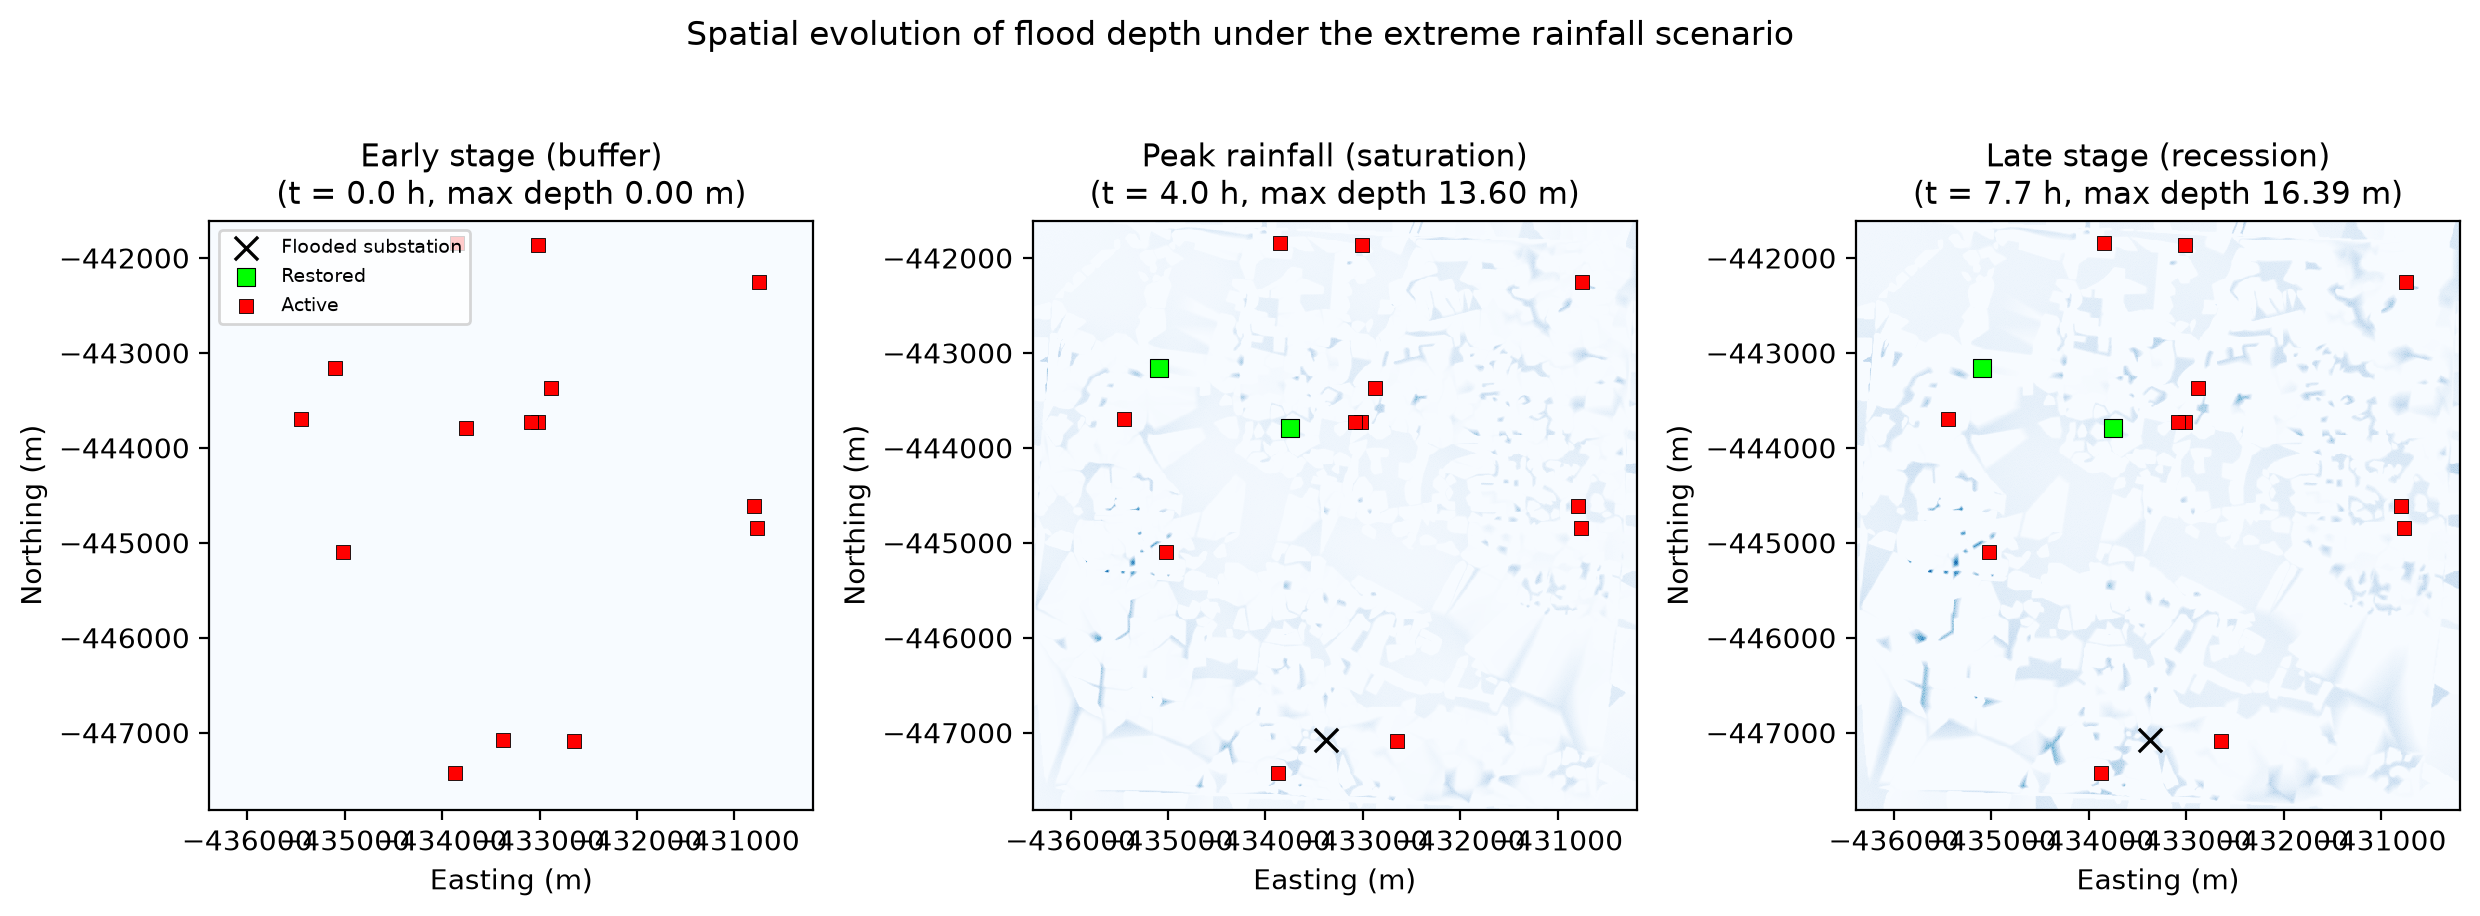
\includegraphics[width=0.95\linewidth]{figures/fig2_flood_evolution.png}
\caption{Spatial evolution of flood depth at different simulation stages under
the extreme rainfall scenario. Flooded substations are marked with black
crosses, restored substations with green squares, and active substations with
red squares.}
\label{fig:flood}
\end{figure}

\subsubsection{Stage I: hydrological buffer period}
During the early rainfall period (approximately the first 2~h), surface
water accumulation remained relatively limited: the maximum depth grew from
0 to about 1.5~m while drainage systems absorbed a large proportion of
incoming water through available storage capacity. This indicates that urban
drainage infrastructure provides a temporary resilience buffer before
reaching saturation.

\subsubsection{Stage II: drainage saturation transition}
As rainfall intensity approached its peak (between 2 and 4~h), subsurface
storage capacity gradually decreased. When $K(i,j,t) \rightarrow 0$, drainage
effectiveness declined significantly and the maximum depth accelerated from
2.8~m at $t=1$~h to 12.6~m at $t=4$~h. The simulation demonstrates that
flood growth is not proportional to rainfall input: once local drainage
capacity is exhausted, additional precipitation rapidly converts into
surface accumulation. This transition represents a critical hydrological
tipping point, consistent with the nonlinear saturation mechanism described
in Section~\ref{sec:method}.

\subsubsection{Stage III: rapid surface flood expansion}
After drainage saturation, flood propagation became dominated by surface
hydraulic exchange, and the peak depth grew further to 16.59~m before slowly
receding. Due to heterogeneous terrain, water preferentially accumulated in
low-elevation regions and river-adjacent areas. Compared with the static
flood approximation (Baseline 1), the proposed CA model captured stronger
spatial concentration of flood depth, particularly in urban depressions.

\subsection{Comparison with the Static Flood Model}
Table~\ref{tab:results} compares the main scenario with the two baselines.
The static bathtub model (Baseline 1) produces a peak flood depth of only
0.48~m and fails to flood any substation, whereas the proposed terrain-informed
CA model reaches a peak depth of 16.59~m and exposes up to three substations to
flooding. The static approximation underestimates the peak depth by more than
97\%, because it neglects terrain-driven accumulation in local depressions.
This result indicates that spatially homogeneous flood assumptions may
substantially underestimate localized infrastructure exposure, especially in
heterogeneous urban environments.

\begin{table}[H]
\centering
\caption{Summary metrics of the main scenario and baselines}
\label{tab:results}
\begin{tabular}{lcccc}
\toprule
Scenario & Peak depth (m) & Flooded subst.\textsuperscript{a} & Restored subst.\textsuperscript{b} & Failed comm.\textsuperscript{a} \\
\midrule
Proposed framework & 16.59 & 1 & 2 & 1 \\
Baseline 1 (static flood) & 0.48 & 0 & 0 & 0 \\
Baseline 2 (no restoration) & 16.59 & 3 & 0 & 10 \\
\bottomrule
\end{tabular}

\medskip
\footnotesize
\textsuperscript{a}Maximum simultaneous value over the simulation.
\textsuperscript{b}Total substations restored by the end of the simulation.
\end{table}

\subsection{Time-Delayed Cascading Failure Analysis}
The interaction between physical flooding and infrastructure dependency
generates a delayed cascading effect. In the main scenario the first
substation is flooded at approximately $t=2$~h; because of the backup-battery
buffer, however, no communication station fails during the first 6~h of the
event. The simulation shows three characteristic phases: (i) physical damage
accumulation; (ii) battery-supported resilience buffering; and (iii)
accelerated communication failure after battery depletion. In the
no-restoration baseline the first communication failures emerge at
$t\approx 6.7$~h and the number of failed stations grows to ten by the end of
the event. This demonstrates that infrastructure resilience cannot be
evaluated solely from immediate physical damage: temporal redundancy
significantly influences the observed failure trajectory
~\cite{ouyang2012time,panteli2015grid}.

\subsection{Effectiveness of the Dynamic Restoration Strategy}
The proposed restoration strategy was compared with the no-intervention
scenario (Baseline 2). Fig.~\ref{fig:resilience} shows the resilience
trajectories $\Phi(t)$ of the three scenarios. Without restoration, the
communication network degrades progressively as batteries deplete, reaching
$\Phi = 0.75$ with ten failed stations. With dynamic dispatch, both repair
fleets restore two flooded substations within the first 3.3~h of the event,
limiting communication failures to a single station and maintaining
$\Phi \ge 0.975$ throughout; the resilience area under the curve improves
from 0.951 to 0.996. The results demonstrate that restoration timing and
target selection strongly influence final system resilience.

\begin{figure}[H]
\centering
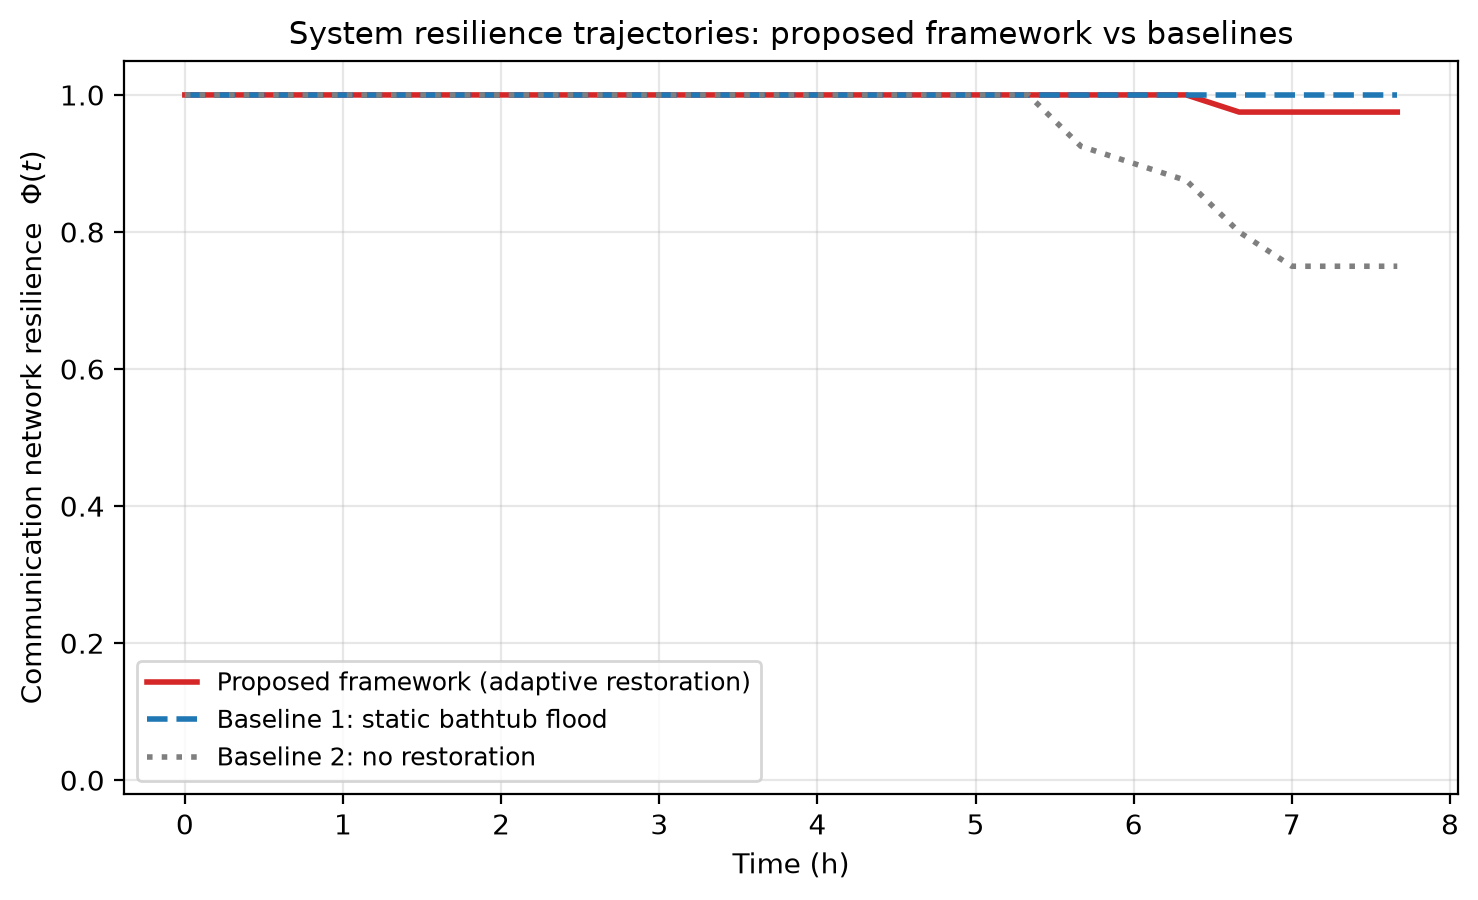
\includegraphics[width=0.88\linewidth]{figures/fig3_resilience_curves.png}
\caption{Communication network resilience trajectories $\Phi(t)$ of the
proposed framework and the two baselines.}
\label{fig:resilience}
\end{figure}

\subsection{Sensitivity Analysis}
One-at-a-time sensitivity experiments were conducted to evaluate the
influence of four key parameters: rainfall intensity, drainage capacity,
backup-battery duration, and the number of repair fleets
(Fig.~\ref{fig:sensitivity}).

Rainfall intensity has a direct and significant effect on flood severity:
increasing the peak intensity from 70 to 100 to 130~mm/h raises the peak
flood depth from 15.14 to 16.59 to 19.91~m (an approximately 31\% increase
in depth for a 30\% increase in rainfall at the highest level).

The drainage-capacity experiments reveal an important saturation mechanism:
once the subsurface storage is exhausted during the peak of the event,
further increases in the drainage rate no longer reduce the peak water
depth (16.59~m in all three configurations). This confirms that the
storage-saturation tipping point, rather than the drainage rate itself,
governs peak flooding under extreme rainfall.

Backup-battery duration directly controls the delayed-cascade buffer:
shortening the battery range to 1.5--2.5~h reduces the resilience AUC from
0.996 to 0.989, whereas extending it to 6--8~h completely prevents
communication failures ($\Phi = 1.0$ throughout). Finally, the
repair-fleet experiments show that two fleets suffice to contain the damage
scenario considered here, while a single fleet briefly exposes a second
substation to flooding before it is repaired.

The sensitivity analysis identifies rainfall intensity and backup-battery
duration as the dominant factors controlling urban resilience performance
under the simulated event, and provides quantitative support for
resilience-oriented planning decisions.

\begin{figure}[H]
\centering
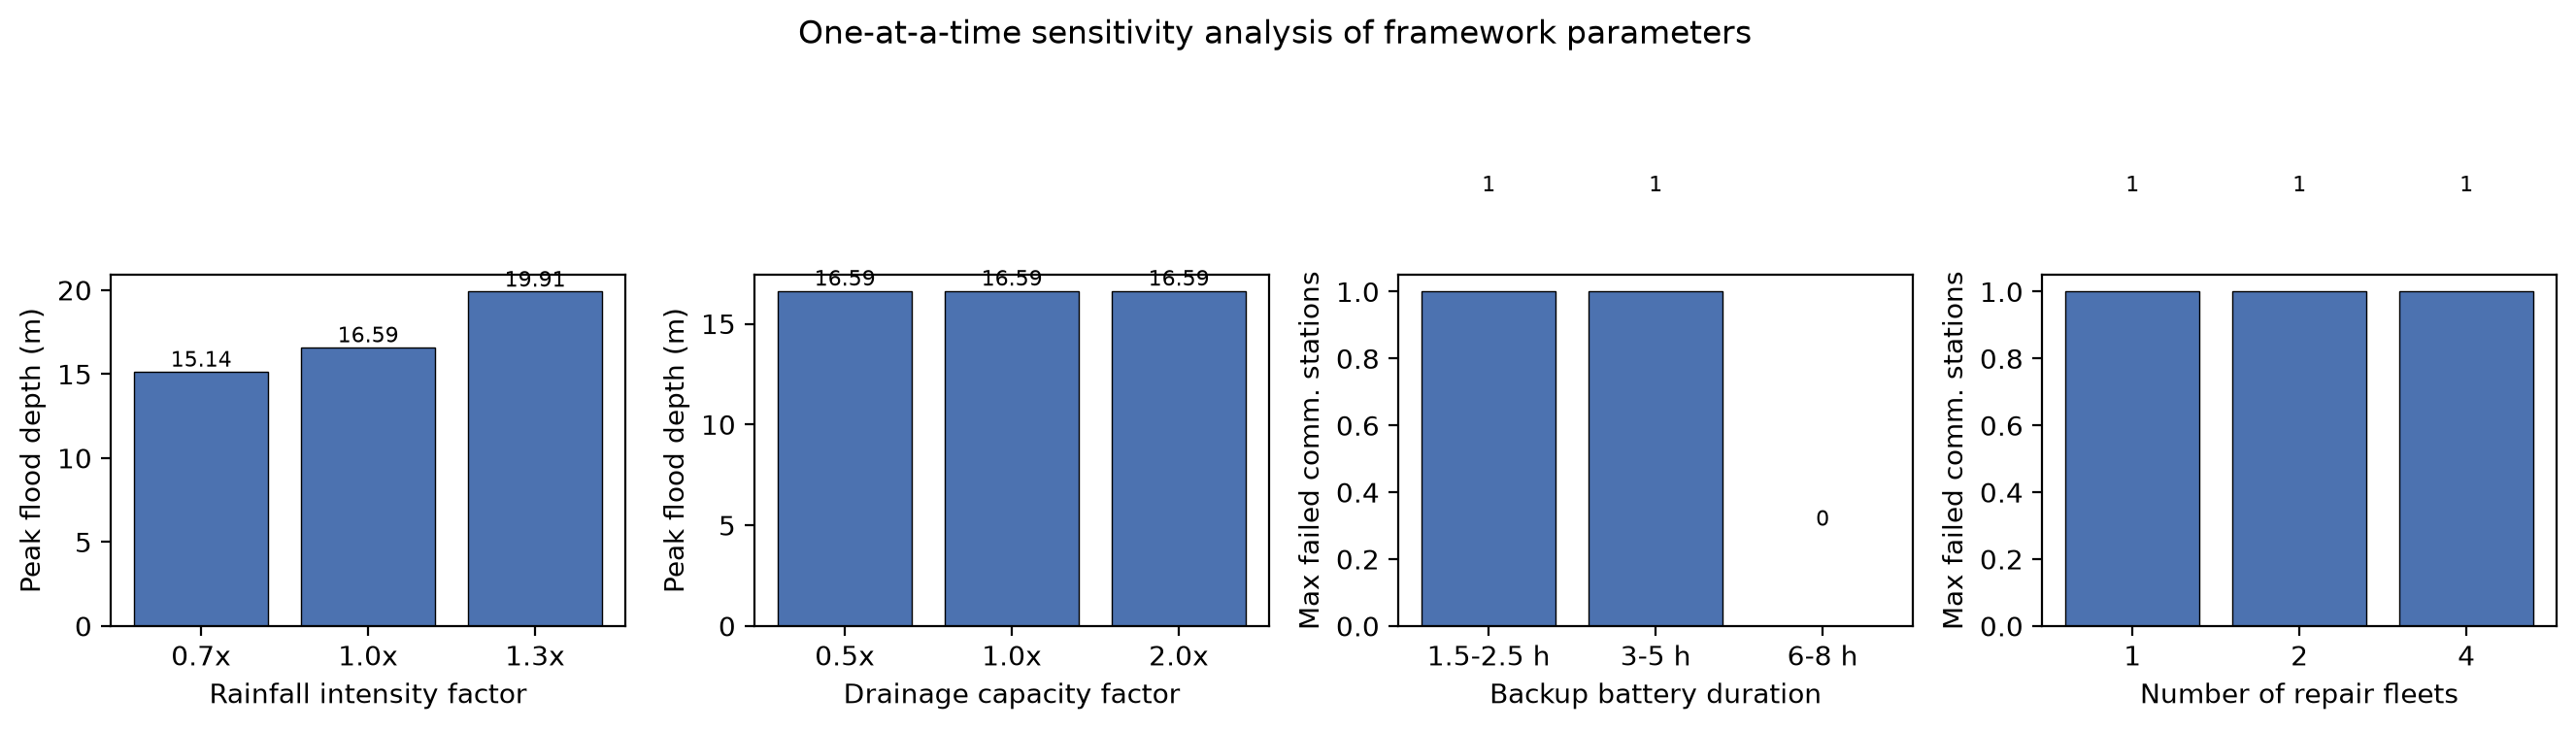
\includegraphics[width=0.95\linewidth]{figures/fig4_sensitivity.png}
\caption{One-at-a-time sensitivity analysis: (a) rainfall intensity vs.\ peak
flood depth; (b) drainage capacity vs.\ peak flood depth; (c) backup-battery
duration vs.\ maximum failed communication stations; (d) number of repair
fleets vs.\ maximum failed communication stations.}
\label{fig:sensitivity}
\end{figure}

\subsection{Summary of Results}
The experimental results demonstrate that the proposed digital twin framework
can simultaneously represent flood dynamics, infrastructure cascading
failures, and adaptive recovery processes. The integration of physics-based
simulation and decision optimization provides a comprehensive approach for
evaluating urban resilience under extreme flooding scenarios.

% =====================================================================
\section{Discussion}\label{sec:discussion}

The proposed digital twin framework provides a unified perspective for
analyzing the interactions among environmental hazards, infrastructure
interdependencies, and emergency responses. Unlike conventional resilience
assessment approaches that primarily focus on static vulnerability
evaluation, this study emphasizes the dynamic evolution of urban systems
under extreme flooding conditions.

\subsection{Implications for Urban Resilience Planning}
The simulation results highlight that urban resilience is determined not only
by the physical robustness of infrastructure components but also by the
temporal characteristics of failure propagation and recovery capability.

First, the nonlinear transition caused by drainage saturation indicates that
flood resilience cannot be evaluated solely according to rainfall intensity
or static elevation information. Urban drainage capacity, terrain
heterogeneity, and local water accumulation processes should be incorporated
into resilience-oriented planning~\cite{bates2010simple,
guidolin2016weighted}.

Second, the time-delayed cascading failure mechanism demonstrates the
importance of operational redundancy. Backup energy systems, such as
batteries and distributed power resources, can significantly extend the
functional lifetime of dependent infrastructure after primary failures
occur~\cite{panteli2015grid}. However, such redundancy should be regarded as
a temporary resilience buffer rather than a permanent solution: in our
simulations the delayed failure merely postpones, but does not eliminate,
the collapse of dependent networks.

Third, the restoration simulation indicates that emergency response
efficiency depends on both infrastructure priority and transportation
accessibility~\cite{laporte2009fifty}. Conventional disaster response
strategies based on static geographic distance may become ineffective when
transportation networks are dynamically disrupted by flooding. Therefore,
future smart-city emergency systems should integrate real-time environmental
sensing, digital twins, and adaptive optimization algorithms
~\cite{batty2018digital,tao2019digital}.

\subsection{Contribution to Digital Twin-Based Disaster Management}
Digital twins have increasingly been applied in smart-city management;
however, many existing implementations focus on monitoring and visualization
rather than predictive resilience analysis~\cite{grieves2017digital,
batty2018digital}. The proposed framework extends the concept of digital
twins by introducing three capabilities: (i) physics-informed environmental
evolution, (ii) multi-layer infrastructure failure simulation, and (iii)
closed-loop human intervention modeling. This enables the digital twin to
function not only as a passive monitoring platform but also as a
decision-support system for disaster mitigation and recovery.

\subsection{Model Limitations and Future Work}
Although the proposed framework improves the representation of flood-induced
infrastructure failures, several limitations remain.

\subsubsection{Hydrodynamic approximation}
The CA-based flood model provides computational efficiency for large-scale
simulations, but it does not fully reproduce all physical processes described
by high-fidelity shallow water equations. In particular, momentum
conservation, turbulence effects, and complex urban obstacles are simplified.
Furthermore, the conservative CFL parameter ($\alpha = 0.12$) limits surface
flow propagation speed, so the reported absolute times represent model time
rather than real physical time; the study focuses on relative timing and the
shape of the transitions rather than exact arrival-time forecasts. Future
research may integrate adaptive mesh refinement, adaptive time stepping, or
hybrid CA--SWE approaches to improve physical accuracy while maintaining
computational efficiency~\cite{bates2010simple}.

\subsubsection{Infrastructure representation}
The current model focuses on power and communication dependencies. However,
real urban systems contain additional interacting layers, including
transportation, water supply, healthcare, and emergency services. Future
studies should extend the framework toward multi-layer infrastructure
networks and incorporate distributed energy resources with self-healing
islanding capabilities~\cite{ouyang2014review}.

\subsubsection{Parameter calibration and validation}
The current simulation relies on parameter settings derived from engineering
assumptions and available geographic information. Further validation using
historical flood observations, sensor measurements, and infrastructure
failure records is required to improve predictive capability. Quantitative
validation metrics such as Intersection over Union (IoU) between simulated
and observed inundation areas should be applied when observational data
become available.

\subsubsection{Human decision modeling}
The emergency dispatch strategy is represented through algorithmic
optimization. However, real disaster response also involves human
decision-making, resource constraints, and institutional coordination
~\cite{dibaldassarre2013socio}. Future work could incorporate agent-based
models to represent more realistic emergency management behaviors.

% =====================================================================
\section{Conclusion}\label{sec:conclusion}

This study proposed a high-resolution digital twin framework for evaluating
urban infrastructure resilience under extreme flooding scenarios. By
integrating terrain-informed cellular automata flood propagation,
time-delayed cascading failure mechanisms, and dynamic restoration
optimization, the proposed framework provides a unified approach for
simulating the complete disaster-response process from hazard evolution to
infrastructure recovery.

The main findings are summarized as follows:
\begin{enumerate}
\item \textbf{Flood evolution exhibits nonlinear transition behavior.} The
interaction between rainfall input, heterogeneous terrain, and drainage
saturation produces critical transition points where urban flooding rapidly
changes from a manageable condition to severe surface accumulation.
\item \textbf{Temporal redundancy strongly influences cascading failure
dynamics.} Backup energy systems introduce a delay between physical
infrastructure damage and functional service disruption. Ignoring this
temporal mechanism may lead to inaccurate estimation of infrastructure
resilience.
\item \textbf{Adaptive restoration improves system-level resilience.}
Dynamic dispatch strategies considering both infrastructure importance and
flood-constrained accessibility can effectively reduce cascading impacts and
improve recovery outcomes under limited emergency resources.
\end{enumerate}

From a methodological perspective, the framework bridges physical flood
dynamics, infrastructure dependency modeling, and recovery optimization
within a unified computational environment. From a practical perspective, it
provides evidence-based support for urban resilience planning by identifying
critical infrastructure vulnerabilities, evaluating cascading impacts, and
testing adaptive intervention strategies. Overall, this research demonstrates
the potential of high-resolution digital twins as a foundation for future
intelligent disaster management systems that combine physical simulation,
network science, and adaptive decision-making.

% =====================================================================
\section*{Acknowledgements}
This work was supported by [funding information to be completed by the
authors].

\section*{Data Availability}

The input data used in this study are derived from publicly available
third-party sources: the road network of Miyazaki City was obtained from
OpenStreetMap (OSM, \url{https://www.openstreetmap.org}), and terrain
elevation data were retrieved from the Open-Meteo elevation API
(\url{https://open-meteo.com}). No proprietary or confidential data were
used.

The complete simulation framework, including the terrain-informed cellular
flood model, the interdependent infrastructure failure model, the adaptive
restoration optimizer, and the visualization modules, is implemented in
Python. All source code, configuration files, cached input data, and the
full set of experimental outputs (frame-wise simulation trajectories,
summary metrics, and figure-generation scripts) will be made publicly
available in a permanent repository upon acceptance of this manuscript
[repository DOI/link to be inserted]. The entire experimental pipeline,
including the main scenario, the two baseline scenarios, and the
one-at-a-time sensitivity analysis, is fully reproducible by executing the
provided scripts with the released code and data.

\bibliographystyle{elsarticle-num}
\bibliography{references}

\end{document}
